% !TeX program = pdfLaTeX
\documentclass[12pt]{article}
\usepackage{amsmath}
\usepackage{graphicx,psfrag,epsf}
\usepackage{enumerate}
\usepackage{natbib}
\usepackage{textcomp}
\usepackage[hyphens]{url} % not crucial - just used below for the URL
\usepackage{hyperref}
\providecommand{\tightlist}{%
  \setlength{\itemsep}{0pt}\setlength{\parskip}{0pt}}

%\pdfminorversion=4
% NOTE: To produce blinded version, replace "0" with "1" below.
\newcommand{\blind}{0}

% DON'T change margins - should be 1 inch all around.
\addtolength{\oddsidemargin}{-.5in}%
\addtolength{\evensidemargin}{-.5in}%
\addtolength{\textwidth}{1in}%
\addtolength{\textheight}{1.3in}%
\addtolength{\topmargin}{-.8in}%

%% load any required packages here


\usepackage{color}
\usepackage{fancyvrb}
\newcommand{\VerbBar}{|}
\newcommand{\VERB}{\Verb[commandchars=\\\{\}]}
\DefineVerbatimEnvironment{Highlighting}{Verbatim}{commandchars=\\\{\}}
% Add ',fontsize=\small' for more characters per line
\usepackage{framed}
\definecolor{shadecolor}{RGB}{248,248,248}
\newenvironment{Shaded}{\begin{snugshade}}{\end{snugshade}}
\newcommand{\AlertTok}[1]{\textcolor[rgb]{0.94,0.16,0.16}{#1}}
\newcommand{\AnnotationTok}[1]{\textcolor[rgb]{0.56,0.35,0.01}{\textbf{\textit{#1}}}}
\newcommand{\AttributeTok}[1]{\textcolor[rgb]{0.77,0.63,0.00}{#1}}
\newcommand{\BaseNTok}[1]{\textcolor[rgb]{0.00,0.00,0.81}{#1}}
\newcommand{\BuiltInTok}[1]{#1}
\newcommand{\CharTok}[1]{\textcolor[rgb]{0.31,0.60,0.02}{#1}}
\newcommand{\CommentTok}[1]{\textcolor[rgb]{0.56,0.35,0.01}{\textit{#1}}}
\newcommand{\CommentVarTok}[1]{\textcolor[rgb]{0.56,0.35,0.01}{\textbf{\textit{#1}}}}
\newcommand{\ConstantTok}[1]{\textcolor[rgb]{0.00,0.00,0.00}{#1}}
\newcommand{\ControlFlowTok}[1]{\textcolor[rgb]{0.13,0.29,0.53}{\textbf{#1}}}
\newcommand{\DataTypeTok}[1]{\textcolor[rgb]{0.13,0.29,0.53}{#1}}
\newcommand{\DecValTok}[1]{\textcolor[rgb]{0.00,0.00,0.81}{#1}}
\newcommand{\DocumentationTok}[1]{\textcolor[rgb]{0.56,0.35,0.01}{\textbf{\textit{#1}}}}
\newcommand{\ErrorTok}[1]{\textcolor[rgb]{0.64,0.00,0.00}{\textbf{#1}}}
\newcommand{\ExtensionTok}[1]{#1}
\newcommand{\FloatTok}[1]{\textcolor[rgb]{0.00,0.00,0.81}{#1}}
\newcommand{\FunctionTok}[1]{\textcolor[rgb]{0.00,0.00,0.00}{#1}}
\newcommand{\ImportTok}[1]{#1}
\newcommand{\InformationTok}[1]{\textcolor[rgb]{0.56,0.35,0.01}{\textbf{\textit{#1}}}}
\newcommand{\KeywordTok}[1]{\textcolor[rgb]{0.13,0.29,0.53}{\textbf{#1}}}
\newcommand{\NormalTok}[1]{#1}
\newcommand{\OperatorTok}[1]{\textcolor[rgb]{0.81,0.36,0.00}{\textbf{#1}}}
\newcommand{\OtherTok}[1]{\textcolor[rgb]{0.56,0.35,0.01}{#1}}
\newcommand{\PreprocessorTok}[1]{\textcolor[rgb]{0.56,0.35,0.01}{\textit{#1}}}
\newcommand{\RegionMarkerTok}[1]{#1}
\newcommand{\SpecialCharTok}[1]{\textcolor[rgb]{0.00,0.00,0.00}{#1}}
\newcommand{\SpecialStringTok}[1]{\textcolor[rgb]{0.31,0.60,0.02}{#1}}
\newcommand{\StringTok}[1]{\textcolor[rgb]{0.31,0.60,0.02}{#1}}
\newcommand{\VariableTok}[1]{\textcolor[rgb]{0.00,0.00,0.00}{#1}}
\newcommand{\VerbatimStringTok}[1]{\textcolor[rgb]{0.31,0.60,0.02}{#1}}
\newcommand{\WarningTok}[1]{\textcolor[rgb]{0.56,0.35,0.01}{\textbf{\textit{#1}}}}



\begin{document}


\def\spacingset#1{\renewcommand{\baselinestretch}%
{#1}\small\normalsize} \spacingset{1}


%%%%%%%%%%%%%%%%%%%%%%%%%%%%%%%%%%%%%%%%%%%%%%%%%%%%%%%%%%%%%%%%%%%%%%%%%%%%%%

\if0\blind
{
  \title{\bf MLE of Mixed Normal Distribution}

  \author{
        Jiarong Feng\footnote{\href{mailto:jiarongf1@uci.edu}{\nolinkurl{jiarongf1@uci.edu}}} \\
    Department of Statistics, University of California, Irvine\\
     and \\     Qi Wang\footnote{\href{mailto:qwang18@uci.edu}{\nolinkurl{qwang18@uci.edu}}} \\
    Department of Statistics, University of California, Irvine\\
      }
  \maketitle
} \fi

\if1\blind
{
  \bigskip
  \bigskip
  \bigskip
  \begin{center}
    {\LARGE\bf MLE of Mixed Normal Distribution}
  \end{center}
  \medskip
} \fi

\bigskip
\begin{abstract}
This algorithm allow you to use Newton's Method to calculate the MLE of
one of the means of the two normal distirbuiton, given the percentage
\(\theta\), standard error \(\sigma_1\), \(\sigma_2\), data set Y, and
one of the mean \(\mu_i, i=1,2\). We are using Newton's Method, after
calculating the score function of the likelihood and get the root of
score function to check where will the iteration converge. After we find
the domain of convergence, we also need to check the second derivative
of the root, to make sure that we are getting the maximum value but not
something else of the likelihood function.
\end{abstract}

\noindent%
{\it Keywords:} Mixed Normal Distribution, MLE, Newton's Method, Score
Functionn
\vfill

\newpage
\spacingset{1.45} % DON'T change the spacing!

\section{Introduction to Mixed Normal Distribution}

Mixed normal distribution is made up with two normal distribution, and
with some percent of each of them.

The pdf of this new distribution is like:
\[ p(y_i|\theta)=\theta\phi(y_i;\mu_1,\sigma_1^2) + (1-\theta)\phi(y_i;\mu_2,\sigma_2^2)\]
And here \(\phi(y_i;\mu_i,\sigma_i^2)\) is the normal pdf, which means
that:
\[\phi(y_i;\mu_i,\sigma_i^2)=\frac{1}{\sqrt{2\pi\sigma^2}}exp(-\frac{(y_i-\mu_i)^2}{-2\sigma_i^2})\]

Our goal is to calculate the MLE of \(\mu_1\) given the other
\(\mu_2, \theta, \sigma_1 \ and \ \sigma_2\)

\section{Code}

\begin{Shaded}
\begin{Highlighting}[]
\NormalTok{g \textless{}{-}}\StringTok{ }\ControlFlowTok{function}\NormalTok{(y, theta, mu\_}\DecValTok{1}\NormalTok{, mu\_}\DecValTok{2}\NormalTok{, sigma\_}\DecValTok{1}\NormalTok{, sigma\_}\DecValTok{2}\NormalTok{)\{}
  
\NormalTok{  score \textless{}{-}}\StringTok{ }\KeywordTok{rep}\NormalTok{(}\OtherTok{NA}\NormalTok{,}\KeywordTok{length}\NormalTok{(y))}
  
  \ControlFlowTok{for}\NormalTok{(i }\ControlFlowTok{in} \DecValTok{1}\OperatorTok{:}\KeywordTok{length}\NormalTok{(y))\{}
    
\NormalTok{    score[i] \textless{}{-}}\StringTok{ }\NormalTok{( (theta}\OperatorTok{*}\NormalTok{(y[i] }\OperatorTok{{-}}\StringTok{ }\NormalTok{mu\_}\DecValTok{1}\NormalTok{)}\OperatorTok{/}\NormalTok{sigma\_}\DecValTok{1}\OperatorTok{\^{}}\DecValTok{2}\NormalTok{)}\OperatorTok{*}\KeywordTok{dnorm}\NormalTok{(y[i], mu\_}\DecValTok{1}\NormalTok{, sigma\_}\DecValTok{1}\NormalTok{ ) ) }\OperatorTok{/}\StringTok{ }
\StringTok{      }\NormalTok{( (theta}\OperatorTok{*}\StringTok{ }\KeywordTok{dnorm}\NormalTok{(y[i], mu\_}\DecValTok{1}\NormalTok{, sigma\_}\DecValTok{1}\NormalTok{ )) }\OperatorTok{+}\StringTok{ }\NormalTok{(}\DecValTok{1}\OperatorTok{{-}}\NormalTok{theta)}\OperatorTok{*}\KeywordTok{dnorm}\NormalTok{(y[i], mu\_}\DecValTok{2}\NormalTok{, sigma\_}\DecValTok{2}\NormalTok{) )}

\NormalTok{  \}}
  
  \KeywordTok{return}\NormalTok{(}\KeywordTok{sum}\NormalTok{(score))}
\NormalTok{\}}

\NormalTok{deriv\_g \textless{}{-}}\StringTok{ }\ControlFlowTok{function}\NormalTok{(y, theta, mu\_}\DecValTok{1}\NormalTok{ , mu\_}\DecValTok{2}\NormalTok{, sigma\_}\DecValTok{1}\NormalTok{, sigma\_}\DecValTok{2}\NormalTok{, }\DataTypeTok{h =} \FloatTok{1e{-}2}\NormalTok{)\{}
  
\NormalTok{   derivative \textless{}{-}}\StringTok{ }\NormalTok{(}\KeywordTok{g}\NormalTok{(y, theta, mu\_}\DecValTok{1}\OperatorTok{+}\NormalTok{h , mu\_}\DecValTok{2}\NormalTok{, sigma\_}\DecValTok{1}\NormalTok{, sigma\_}\DecValTok{2}\NormalTok{)}\OperatorTok{{-}}\StringTok{ }
\StringTok{                    }\KeywordTok{g}\NormalTok{(y, theta, mu\_}\DecValTok{1}\OperatorTok{{-}}\NormalTok{h , mu\_}\DecValTok{2}\NormalTok{, sigma\_}\DecValTok{1}\NormalTok{, sigma\_}\DecValTok{2}\NormalTok{))}\OperatorTok{/}\NormalTok{(}\DecValTok{2}\OperatorTok{*}\NormalTok{h)}
   
   \KeywordTok{return}\NormalTok{(derivative)}
\NormalTok{\}}
  
\NormalTok{mixture\_normal.mle \textless{}{-}}\StringTok{ }\ControlFlowTok{function}\NormalTok{(y, theta, mu\_}\DecValTok{1}\NormalTok{, mu\_}\DecValTok{2}\NormalTok{, sigma\_}\DecValTok{1}\NormalTok{, sigma\_}\DecValTok{2}\NormalTok{,}
                               \DataTypeTok{max.iter =} \DecValTok{1000}\NormalTok{, }\DataTypeTok{small =} \FloatTok{1e{-}3}\NormalTok{, }\DataTypeTok{h =} \FloatTok{1e{-}2}\NormalTok{)\{}
  
  \ControlFlowTok{for}\NormalTok{(iter }\ControlFlowTok{in} \DecValTok{1}\OperatorTok{:}\NormalTok{max.iter)\{}
\NormalTok{    mu\_}\FloatTok{1.}\NormalTok{old \textless{}{-}}\StringTok{ }\NormalTok{mu\_}\DecValTok{1}
\NormalTok{    mu\_}\DecValTok{1}\NormalTok{ \textless{}{-}}\StringTok{ }\NormalTok{mu\_}\FloatTok{1.}\NormalTok{old }\OperatorTok{{-}}\StringTok{ }\KeywordTok{g}\NormalTok{(y,theta,mu\_}\FloatTok{1.}\NormalTok{old, mu\_}\DecValTok{2}\NormalTok{, sigma\_}\DecValTok{1}\NormalTok{, sigma\_}\DecValTok{2}\NormalTok{)}\OperatorTok{/}
\StringTok{      }\KeywordTok{deriv\_g}\NormalTok{(y,theta,mu\_}\FloatTok{1.}\NormalTok{old, mu\_}\DecValTok{2}\NormalTok{, sigma\_}\DecValTok{1}\NormalTok{, sigma\_}\DecValTok{2}\NormalTok{, h)}
    
    \ControlFlowTok{if}\NormalTok{(}\KeywordTok{abs}\NormalTok{(mu\_}\FloatTok{1.}\NormalTok{old }\OperatorTok{{-}}\StringTok{ }\NormalTok{mu\_}\DecValTok{1}\NormalTok{) }\OperatorTok{\textless{}=}\StringTok{ }\NormalTok{small)}
      \ControlFlowTok{break}
\NormalTok{  \}}
    
\NormalTok{  out \textless{}{-}}\StringTok{ }\KeywordTok{list}\NormalTok{(mu\_}\DecValTok{1}\NormalTok{, iter, iter }\OperatorTok{!=}\StringTok{ }\NormalTok{max.iter)}
  \KeywordTok{names}\NormalTok{(out) \textless{}{-}}\StringTok{ }\KeywordTok{c}\NormalTok{(}\StringTok{"MLE"}\NormalTok{, }\StringTok{"iteration.count"}\NormalTok{, }\StringTok{"converge"}\NormalTok{)}
\NormalTok{  out}
\NormalTok{\}}


\NormalTok{y \textless{}{-}}\StringTok{ }\KeywordTok{c}\NormalTok{(}\FloatTok{8.1}\NormalTok{, }\FloatTok{8.2}\NormalTok{, }\FloatTok{8.1}\NormalTok{, }\FloatTok{8.2}\NormalTok{, }\FloatTok{8.2}\NormalTok{, }\FloatTok{7.4}\NormalTok{, }\FloatTok{7.3}\NormalTok{, }\FloatTok{7.4}\NormalTok{, }\FloatTok{8.1}\NormalTok{, }
       \FloatTok{8.1}\NormalTok{, }\FloatTok{7.9}\NormalTok{, }\FloatTok{7.8}\NormalTok{, }\FloatTok{8.2}\NormalTok{, }\FloatTok{7.9}\NormalTok{, }\FloatTok{7.9}\NormalTok{, }\FloatTok{8.1}\NormalTok{, }\FloatTok{8.1}\NormalTok{)}
\end{Highlighting}
\end{Shaded}

Here we used a dataset y to verify whether we have the right MLE, since
Newton's method is unstable, sensitive to the initial point.

\section{Test whether score function is wrong}

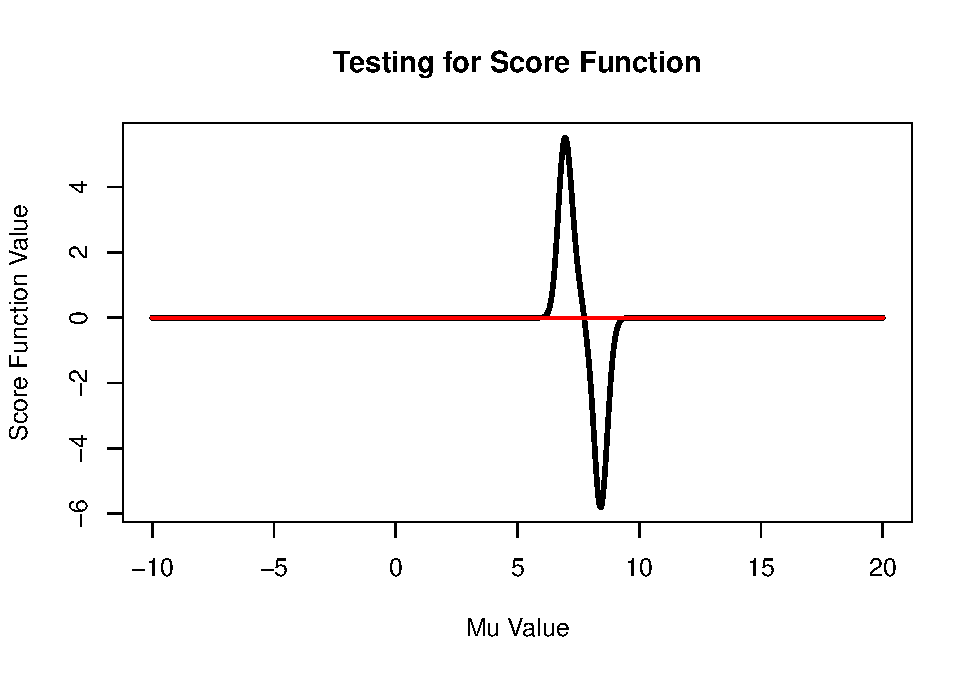
\includegraphics{Mixed_Normal_MLE_files/figure-latex/unnamed-chunk-2-1.pdf}

It seems that there are many many zero points. Don't forget we are using
the zero point of score function to calculate the MLE!

\section{Test whether derivative of score function is wrong}

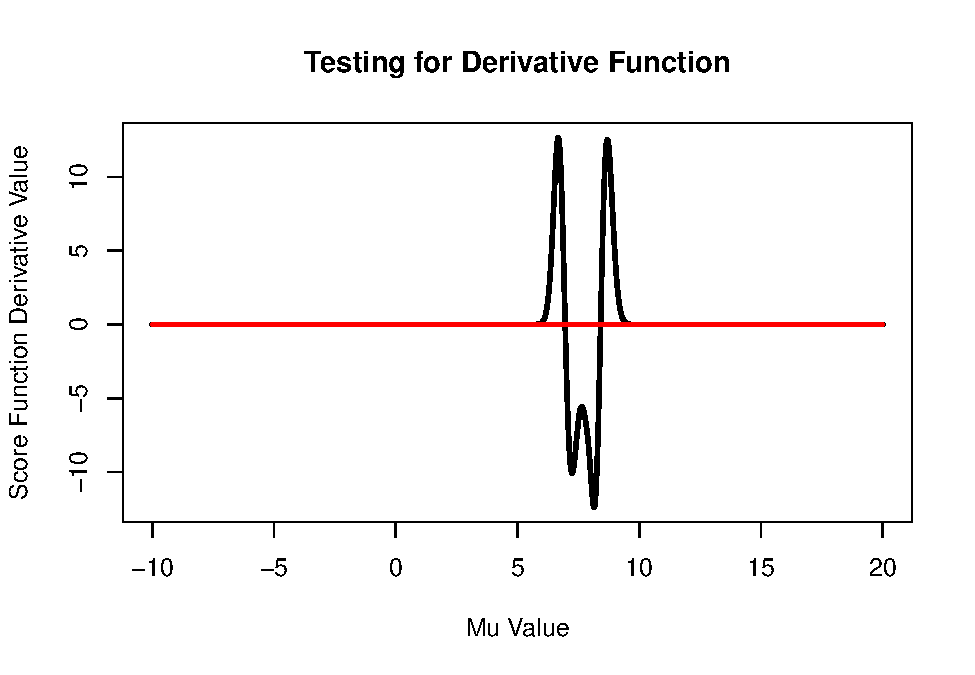
\includegraphics{Mixed_Normal_MLE_files/figure-latex/unnamed-chunk-3-1.pdf}
According to the definition of second derivative, and first derivative,
the function has the maximum value when the first derivative is near 8.
Because the LLH function value has been increasing until that point.
Also, the second derivative is negative according to picture 2. So the
Derivative function is also right. \textbf{But we notice that, only when
\(mu_1\) is between 5 and 10, will the second derivative not equal to
0.}

\section{Chosing Initialization Values and Calculate Domain of Convergence}

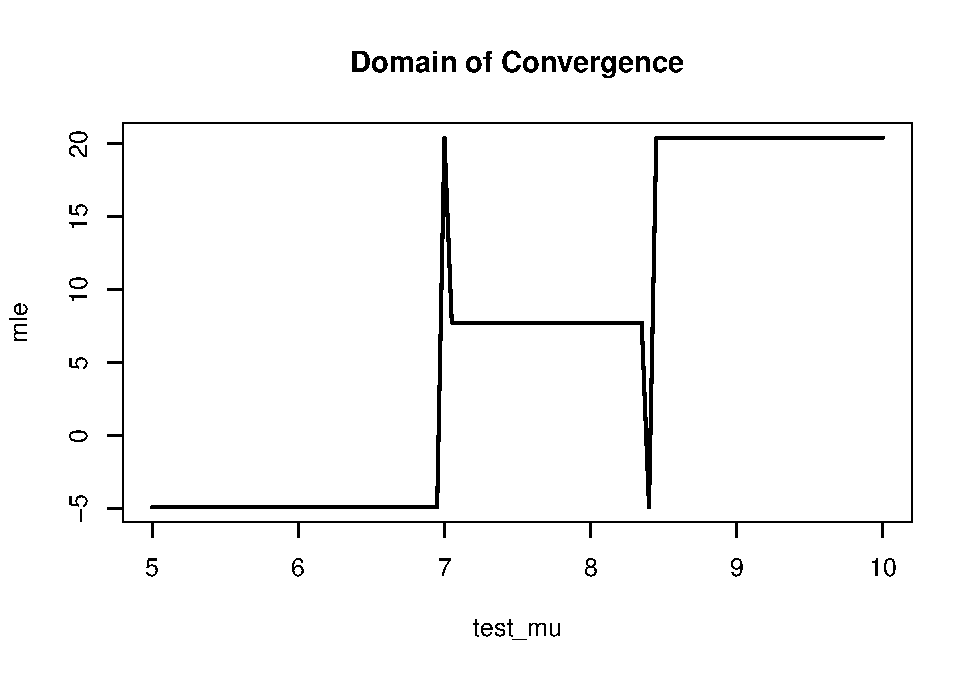
\includegraphics{Mixed_Normal_MLE_files/figure-latex/unnamed-chunk-4-1.pdf}
It seems right since there is a stable area in -5,8 and 20. So the
domain of convergence for them are obvious. However, there are many
special points around 7 and 8.35. Why are they there? I set the sequence
break to be 0.05, but I need to dig more into them to check what
happened as test\_mu changed from 6.95 to 7.

\section{Special Points}

Around 7:

When I type in the code as follows:

test\_mu\_7 = seq(6.95,7,0.001)\\
mle\_7 = vector()\\
for (i in 1:length(test\_mu\_7))\{\\
mle\_7{[}i{]} = mixture\_normal.mle(y, theta = 0.2, mu\_1 =
test\_mu\_7{[}i{]}, mu\_2 = 8.0, sigma\_1 = sqrt(0.1), sigma\_2 =
sqrt(0.1))\$``MLE''\\
\}\\
plot(x = test\_mu\_7, y = mle\_7, lwd = 2, type = `l')

Error in if (abs(mu\_1.old - mu\_1) \textless= small) break :\\
需要TRUE/FALSE值的地方不可以用缺少值

This might be caused by the special case near 7, leading to the
derivatives hard to calculate! Please check the score function, which is
the derivative for MLE, around 7, it seems that the function is not
differenciable. Similar around 8.

\section{Conclusion}

\begin{enumerate}
\def\labelenumi{\arabic{enumi}.}
\tightlist
\item
  Change and adjust the precision(you named it as ``small''), and
  h(which is used to calculate second derivative for log-likelihood
  function).\\
\item
  Choose initialization value of \(\mu_1\) a little far from the place
  that is not differenciable.
\end{enumerate}

\bibliographystyle{agsm}
\bibliography{bibliography.bib}

\end{document}
